\newpage
\chapter{Planning}

\textsl{This chapter describes the project development model and a plan of the activities and show their dependencies.}

\section{Life-cycle model}

The chosen life-cycle model is the incremental model and it has the following characteristics:

\begin{enumerate}  
	\item Architectural Analysis and Design activities are not repeated: the goal is to spend sufficient time studying the problem and gathering all the requirements so that the architecture of the system is can be fully identified during the initial stages of the project. This allows for a stronger planning;
	\item The implementation of the different parts of the system is incremental and is also planned in the initial stages of the project;
	\item The activities of Design, Coding and Verification are repeated in order to improve existing parts of the system, correct mistakes or add new features;
	\item Maintenance is a continuous activity and aims at making the product solid and bug free.
\end{enumerate}

The advantages of using this model are that the requirements are treated according to their strategic importance and the implementation starts from the primary ones. Furthermore, each increment adds new functionality to the baseline and allows the costumer to frequently test the product prototype and give valuable feedback. By using the evaluations of the customer, every successive iteration of the application should become more complete, converging to an appropriate final version of the product.


\begin{figure}[H]
	\centering
	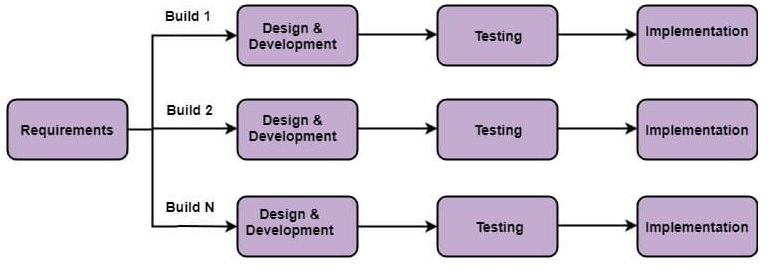
\includegraphics[scale=0.8]{img/incremental.jpg}
	\caption{Incremental Model}
\end{figure} 



\newpage
\section{Gantt chart}
The following chart shows the planification of all the activities involved in the project:

\begin{figure}[H]
	\centering
	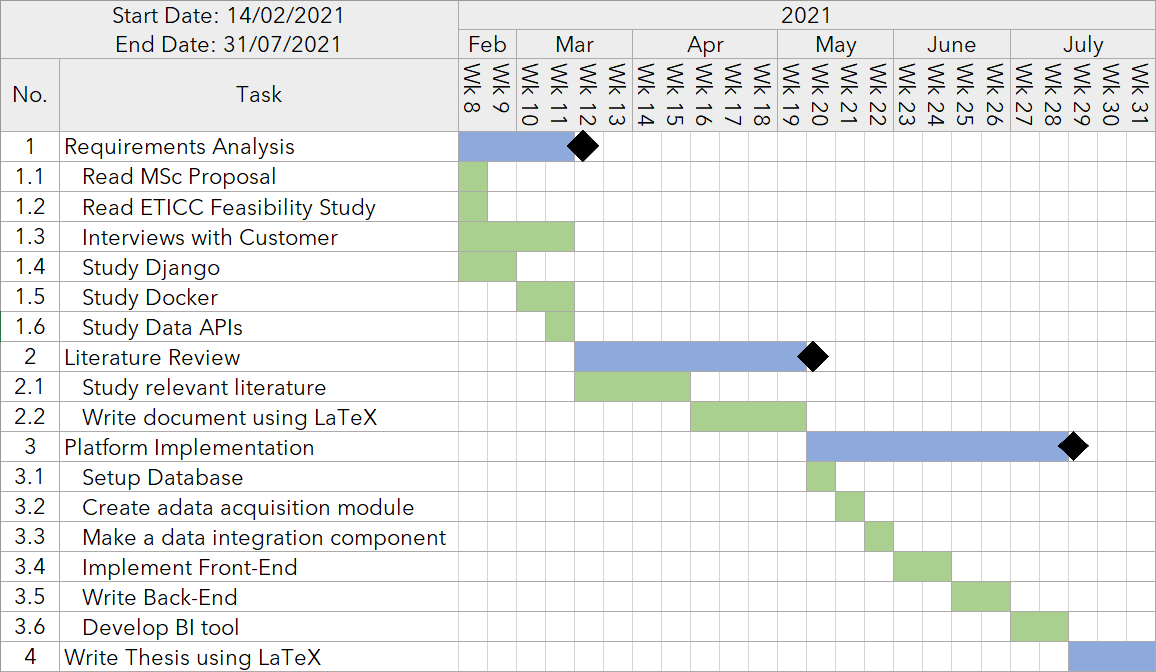
\includegraphics[scale=0.55]{img/gantt.png}
	\caption{Gantt Chart}
\end{figure} 
